%! Author = lazza
%! Date = 10/04/2022

% Preamble
\documentclass[9pt, twocolumn, twoside]{article}

% Packages
\usepackage[a4paper, total={7in, 10in}]{geometry}\usepackage{amsmath}
\usepackage{graphicx}
\usepackage{textcomp}
\usepackage[utf8]{inputenc}
\usepackage[T1]{fontenc}
\usepackage{enumitem}
\usepackage{booktabs}
\usepackage{bitset}
\usepackage{xcolor}
\usepackage{color}
\usepackage{intcalc}
\usepackage{float}
\usepackage{amsfonts}
%\usepackage{latexsymb}

%\title{Advanced Computer Architecture \\ \large Professor Marco D. Santambrogio}
%\author{Gabriele Lazzarelli}
%\date{2022}

\begin{document}
    %\maketitle
    %\noindent\makebox[\textwidth]{
\includegraphics[width= 8cm]{images/LogoPolimi.png}}

    \tableofcontents
    \clearpage

    %%! Author = lazza
%! Date = 10/04/2022

% Preamble
\documentclass[11pt]{article}

% Packages
\usepackage{amsmath}

% Document
\begin{document}
    \section{Introduction}\label{sec:introduction}


    \subsection{Taxonomy}\label{subsec:taxonomy}

    \subsection{Parallelism}\label{subsec:parallelism}

    \subsubsection{Instruction level}
    \subsubsection{Thread level}
    \subsubsection{Both SMT}
    \subsubsection{Heterogeneous}


    \subsection{Heterogeneous systems}\label{subsec:heterogeneous-systems}



\end{document}
    %! Author = lazza
%! Date = 09/05/2022

\section{Performance and Cost}\label{sec:performance-and-cost}
When we say that one computer is faster than another what do we mean?
It depends on what is important.

Two metrics:
\begin{description}
    \item[Computer system user] minimize elapsed time for program execution:\\
    \textbf{latency:} (response time) execution time = time\_end - time\_start
    \item[Computer center manager] maximize completion rate \(=\frac{\#jobs}{\sec}\)\\
    \textbf{throughput:} total amount of work done in a given time
\end{description}
Throughput \(= \frac{1}{latency}\) only if there is not overlap between instructions, otherwise throughput >
response time.

\subsection{Measures}\label{subsec:measures}
\begin{gather*}
    \text{"X is k\% faster than Y"} = \frac{\text{execution time (y)}}{\text{execution time (x)}} = 1 + \frac{n}{100}\\
    \text{\textbf{Performance (x)}} = \frac{1}{\text{execution time(x)}}\\
    \Rightarrow \text{"X is k\% faster than Y"} = \frac{\text{performance (x)}}{\text{performance (y)}} = 1 +
\frac{n}{100}\\
\end{gather*}

\[\text{\textbf{Speed up (x,y)}} = \frac{\text{performance (x)}}{\text{performance (y)}}\]

\subsection{Amdahl's Law}\label{subsec:amdahl's-law}
Suppose that an enhancement E accelerates a fraction F of the task by a factor S (speedup enhanced), and the remainder
of the task in unaffected.

\begin{figure}[H]
    \centering
    
\includegraphics[scale = 0.3]{images/amdahls-law}
    \caption{In green the (F) fraction enhanced.}
    \label{fig:amdalhs-law}
\end{figure}

\begin{gather*}
    ExTime_{new} = ExTime_{old} \times \left( \left( 1 - F_{en} \right) +
\frac{F_{en}}{S_{en}} \right)\\
    \mathbf{S_{overall}} = \frac{ExTime_{old}}{ExTime_{new}} = \frac{1}{\left( 1-F_{en} \right) +
\frac{F_{en}}{S_{en}}}\\
    \mathbf{Speedup_{overall(max)}} = \frac{1}{\left( 1 - F_{en} \right)}\\
\end{gather*}

This means that if an enhancement is only usable for a fraction
of a task we can’t speed up the task by more
than the reciprocal of 1 minus the fraction.
An upgrade is worth it if \(costs < speedup_{overall}\).

\textbf{Note:} in case of threads:
\[\mathbf{Speedup_{overall}} = \frac{1}{s + \frac{p}{N}}\\\]
s = serial part = 1 - Fraction enhanced\\
p = 1 - s = parallelized part = Fraction enhanced\\
N = number of processors or threads = Speedup


\subsection{CPU time and CPI}\label{subsec:cpu-time-and-cpi}
For computer architects:
\begin{center}
    Response time = CPU time + I/O wait
\end{center}

The \textbf{CPU time} does not include I/O wait time and corresponds to the time spent running the program.

\begin{center}
    \begin{align*}
        \text{CPU time (P)} &= \frac{\text{cc needed to execute P}}{\text{clock frequency}}\\
                     &= \text{cc needed to execute P} \times \text{cc time}
    \end{align*}
\end{center}

\begin{center}
    \textbf{CPI} \(=\frac{cycles}{instruction}\)
\end{center}

\begin{center}
    \textbf{IC} \(=\frac{instructions}{program}\)
\end{center}

\begin{center}
    \textbf{Cycle Time} \(=\frac{time}{seconds}\)
\end{center}

\begin{center}
    \textbf{CPU time} \(= IC \times CPI \times Cycle\_Time = \frac{seconds}{program}\)
\end{center}

\subsection{MIPS and MFLOPS}\label{subsec:mips-and-mflops}
MIPS has its shortcomings: it counts every instruction as if they were all equal, CPI varies with different
instructions.
\begin{align*}
    \text{\textbf{MIPS}} &= \text{millions of instructions per second}\\
                         &= \frac{\text{number of instructions}}{\text{execution time} \times 10^6}\\
                         &= \frac{\text{clock frequency}}{\text{CPI}\times 10^6}
\end{align*}

MFLOPS takes care of the problems related to MIPS and considers only the number of floating point operations, which we
assume
independent from compiler and ISA.

\begin{center}
    \textbf{MFLOPS} \(= \frac{\text{Floating point operations in program}}{\text{CPU time} \times 10^6}\)
\end{center}

    %! Author = lazza
%! Date = 11/04/2022

\section{Pipeline}\label{sec:pipeline}

\subsection{MIPS}\label{subsec:heterogeneous-systems}
The MIPS architecture is based on the SIMD model, the instruction set (ISA) is based on 32-bit format instruction.
\begin{figure}[h]
    \centering
    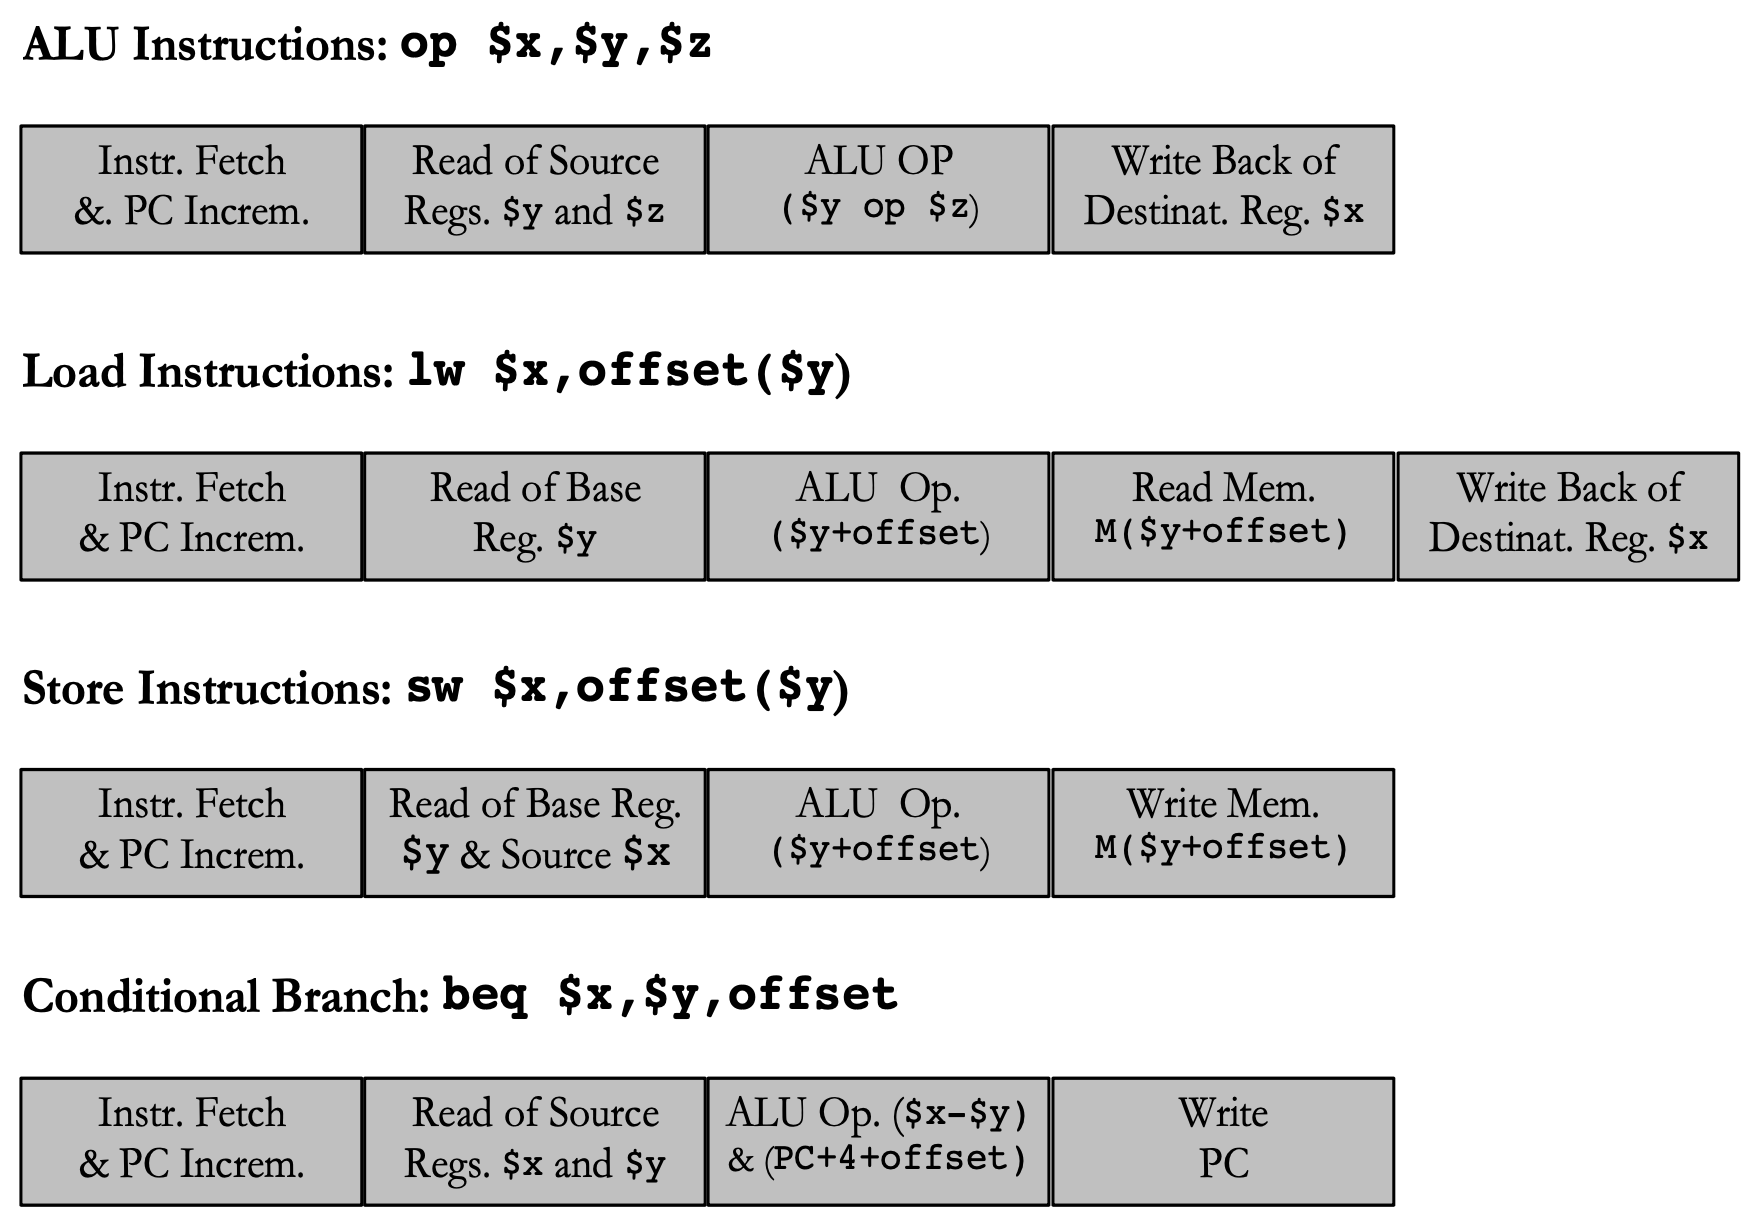
\includegraphics[scale=0.3]{images/MIPS-instructions}
    \caption{MIPS instructions}
    \label{fig: MIPS instructions}
\end{figure}

The CPU, central process unit, amounts to a control unit plus a data path.
Communication between the CPU and the memory in the computing infrastructure happens through the control, data and
address buses.

\begin{figure}[h]
    \centering
    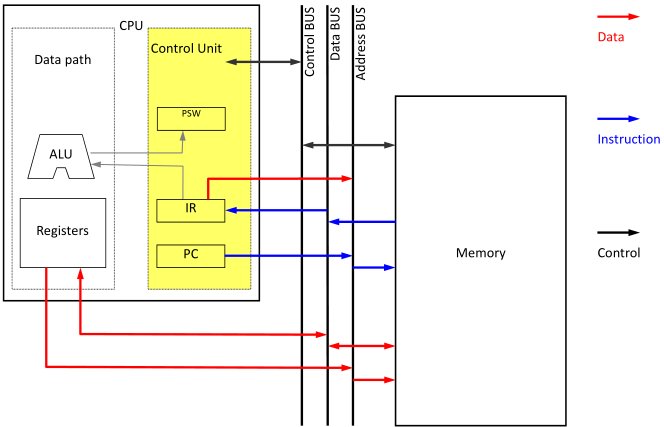
\includegraphics[scale = 0.3]{images/computing-infrastructure}
    \caption{Computing infrastructure}
    \label{fig:computing-infrastructure}
\end{figure}

\paragraph{Execution of MIPS instructions} Every instruction in MIPS subset can be implemented in at most 5 clock
cycles as follows:
\begin{description}
    \item[IF] Instruction Fetch Cycle\\
        Send the content of Program Counter register to Instruction Memory and fetch the
        current instruction from Instruction Memory.

        Update the PC to the next sequential address by adding 4 to the PC (since each instruction is 4 bytes).

    \item[ID] Instruction Decode and Register Read Cycle\\
        Decode the current instruction (fixed-field decoding)
        and read from the Register File of one or two registers
        corresponding to the registers specified in the
        instruction fields.

        Sign-extension of the offset field of the instruction in
        case it is needed.

    \item[EX] Execution Cycle\\
    The ALU operates on the operands prepared in the
    previous cycle depending on the instruction type:
    \begin{itemize}
        \item[-] Register-Register ALU Instructions: ALU executes the specified operation on the operands read
        from the RF
        \item[-] Register-Immediate ALU Instructions:
        ALU executes the specified operation on the first operand
        read from the RF and the sign-extended immediate operand
        \item[-] Memory Reference:
        ALU adds the base register and the offset to calculate the
        effective address.
        \item[-] Conditional branches:
        Compare the two registers read from RF and compute the
        possible branch target address by adding the sign-
        extended offset to the incremented PC\@.
    \end{itemize}


    \item[ME] Memory Access\\
        Load instructions require a read access to the Data
        Memory using the effective address.

        Store instructions require a write access to the Data
        Memory using the effective address to write the data
        from the source register read from the RF\@.

        Conditional branches can update the content of the PC
        with the branch target address, if the conditional test
        yielded true.

    \item[WB] Write-Back Cycle\\
        Load instructions write the data read from memory in
        the destination register of the RF\@.

        ALU instructions write the ALU results into the
        destination register of the RF\@.
\end{description}


\begin{figure}[h]
    \centering
    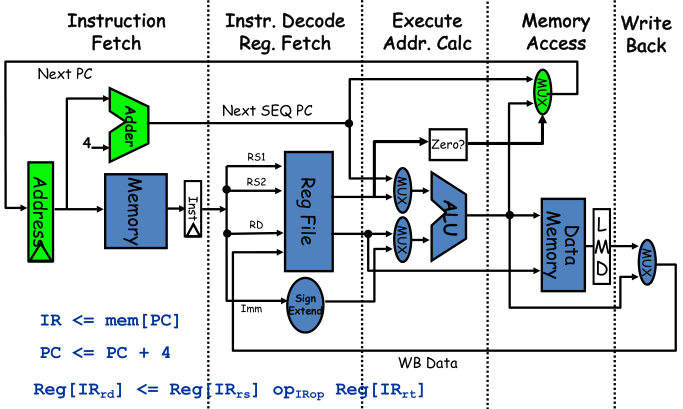
\includegraphics[scale = 0.35]{images/MIPS-data-path}
    \caption{MIPS data path}
    \label{fig:mips-data-path}
\end{figure}

In the single cycle implementation of MIPS the length of the clock cycle is defined by the critical path given by the
load instruction: T = 8ns.
Each instruction is executed in a single clock cycle of 8ns.
\begin{figure}[h]
    \centering
    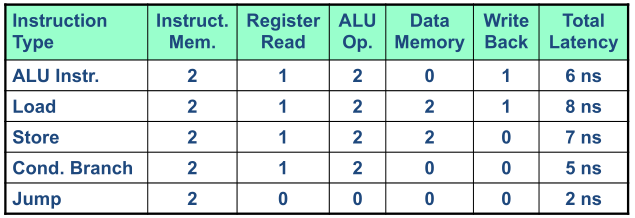
\includegraphics[scale=0.38]{images/instructions-latency}
    \caption{Instruction latency}
    \label{fig:instruction-latency}
\end{figure}

In the multi-cycle implementation the instruction is distributed on multiples cycle (5 for MIPS).

The basic cycle is smaller of 2 ns, the instruction latency is 10 ns.

The multi-cycle execution can be sequential of pipelined.
\begin{figure}[h]
    \centering
    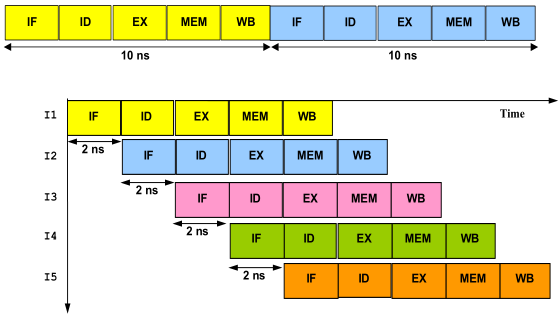
\includegraphics[scale=0.4]{images/sequential-vs-pipelined}
    \caption{Sequential vs pipelined execution}
    \label{fig:sequential-vs-sequential}
\end{figure}

\paragraph{Latency} Each instruction is worsened from 8ns to 10ns.\\
\textbf{Throughput} Is improved by four times, 1 instruction each 8ns to 1 instruction each 2ns.


The Register File is used in WB and ID stages.
In the \textbf{optimized pipeline} the RF-write in the first half of the clock cycle and the RF-read occurs in the
second half of the clock cycle avoiding a possible read after write hazard which otherwise would've required a stall.
It is safely to assume that the optimized pipeline will be the standard pipeline throughout the course.
    %! Author = lazza
%! Date = 02/05/2022

\section{Hazards}\label{sec:hazards}
Dependencies are created at code-level and can be translated into conflicts when the compiler translate the code into
instructions.

A hazard is created whenever there is a conflict (and therefore a dependency) between instructions, and
these instructions are close enough that the overlap caused by pipelining would change the order of access to the
operands involved in the dependence.

Hazards prevent the next instruction in the pipeline from executing during its designated clock cycle, reducing the
performance from the ideal speedup gained by pipelining.

\subsection{Structural hazards}\label{subsec:structural-hazards}
Use of the same resource, such as the ALU, from different instructions simultaneously.
There cannot be structural hazards in the MIPS architecture:
\begin{description}
    \item[] Instruction Memory separated from Data Memory, thus allowing the fetch of instructions and the reading of
    register during the same clock cycle.
    \item[] Register File (RF) can be accessed twice in the same clock cycle: write access on the rising edge of
    the clock and read access on the falling edge by another instruction.
\end{description}

\subsection{Data Hazard}\label{subsec:data-hazard}
Attempt to use a result before it is ready, three different types:
\begin{itemize}
    \item[] RAW, read after write
    \item[] WAR, write after read
    \item[] WAW, write after write
\end{itemize}

\begin{figure}[h]
    \centering
    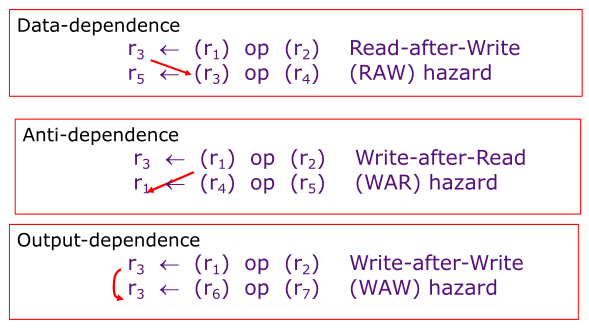
\includegraphics[scale = 0.4]{images/data-hazards-1}
    \caption{Data hazards}
    \label{fig:data-hazards}
\end{figure}


The RAW hazard is the only possible hazard in the MIPS architecture since all five stages are accessed in the
same order in and between instructions, this is due to the fact that in the MIPS architecture there cannot
be simultaneous access to the same resource and the access to the resources follow the order of the instructions.

For this reason write backs are in-order and therefore WAW cannot happen, and the reading of registers of a previous
instruction happens always before the write back of a subsequent instruction precluding the WAR hazards.

RAW hazards can be dealt with at compile-time (design solution) or at run-time (hardware solution).

\paragraph{Compilation Techniques}
\begin{itemize}
    \item[\textrightarrow] Nop instructions, insertion of no operation
    \item[\textrightarrow] Instruction Scheduling, to avoid that correlating instructions are too close the compiler
    tries to insert independent instructions among correlated instructions.
\end{itemize}
Scheduling is a reordering of independent instructions without changing the overall result;
when the compiler does not find independent instructions, it inserts nops.

\paragraph{Hardware Techniques}
\begin{itemize}
    \item[\textrightarrow] Insertion of stalls (or bubbles) in the pipeline
    \item[\textrightarrow] Data Forwarding (or Bypassing)
\end{itemize}

Forwarding data means shortcutting data from one resource of the CPU as output to another resource of the CPU as
input using one clock cycle for the propagation, this means using temporary result stored in the pipeline instead of
waiting for the write back of results in the RF\@.
Forwarding costs are additional multiplexers to allow to fetch inputs from the pipeline.\\
In the MIPS architecture the common paths for data forwarding are EX-EX, MEM-EX, MEM-MEM\@.

Note that WB-ID is not a data path, data is written and accessed in the same clock cycle inside the Register File.
MEM-ID path is not useful if we divide clock cycle in rising and falling edge (optimized pipeline).


\begin{figure}[h]
    \centering
    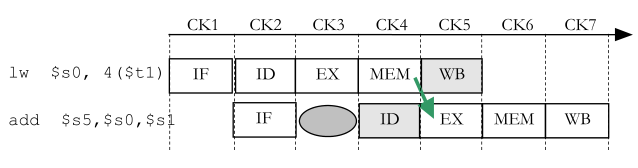
\includegraphics[scale=0.4]{images/load-use-hazard}
    \caption{Load/Use hazard requires a stall to use the MEM-EX path}
    \label{fig:load-use-hazard}
\end{figure}


\begin{figure}[h]
    \centering
    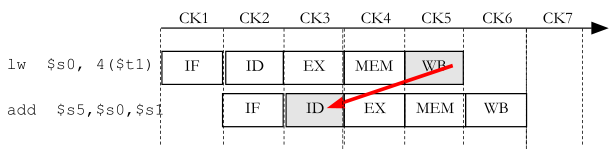
\includegraphics[scale=0.4]{images/load-use-without-forwarding}
    \caption{Load/Use without forwarding needs two stalls}
    \label{fig:load-use-without-forwarding}
\end{figure}


\begin{figure}[h]
    \centering
    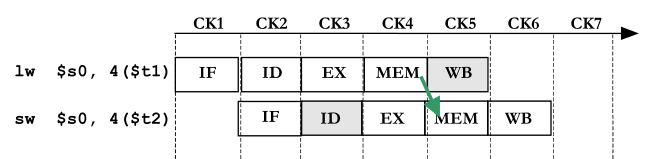
\includegraphics[scale=0.4]{images/load-store-hazard}
    \caption{Load/Store hazard uses the MEM-MEM path}
    \label{fig:load-store-hazard}
\end{figure}


\subsection{Control hazards}\label{subsec:control-hazards}
Attempt to make a decision on the next instruction to execute, before the condition is evaluated.
A MUX is responsible for the value of PC, which is based on ALU output: until the ALU doesn't evaluate the
condition the PC is not known, and we can't know which is the next instruction.

The PC is available at the MEM stage.

Generally true statements are executed in the waiting for the evaluation, as if the condition
were true and no jump was needed: just add to the PC plus one, and then see if the branch is taken.
For this particular reason it is suggested to write inside the \verb|IF| statements the code that most probably is
going to be executed.

In case we wait for the evaluation of the condition the stalls required are two in case of forwarding, three without forwarding.
%add figure explaing

An additional solution would be the early evaluation of the PC in the ID stage instead of the EXE stage, in this new
pipeline the PC adder is anticipated and only one stall would be required (with forwarding) to fetch the correct instruction.
This solution bring an issue in presence of a RAW hazard: anticipating the PC adder means that we have to add a stall
in order to solve the conflict.

\begin{figure}[h]
    \centering
    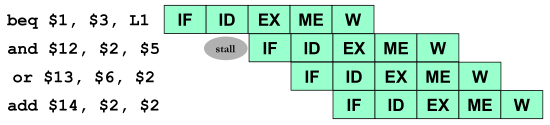
\includegraphics[scale = 0.4]{images/pc-early-evaluation}
    \caption{Early evaluation of the PC}
    \label{fig:pc-early-evaluation}
\end{figure}

\begin{figure}[h]
    \centering
    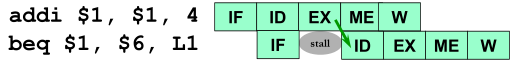
\includegraphics[scale = 0.4]{images/pc-early-evalutation-issue}
    \caption{PC early evaluation issue}
    \label{fig:pc-early-evaluation-issue}
\end{figure}
    %! Author = lazza
%! Date = 02/05/2022

\section{Branch prediction}\label{sec:branch-prediction}
When a branch is taken the \textbf{branch target address} (BTA) is stored in the PC instead of the address of the
next instruction in the sequential instruction stream.
The branch outcome and Branch Target Address are ready at the end of the EX stage, conditional branches are solved
when PC is updated at the end of the ME stage.
Control hazards reduce the performance from the ideal speedup gained by the pipelining since they can
make it necessary to stall the pipeline.

\begin{figure}[h]
    \centering
    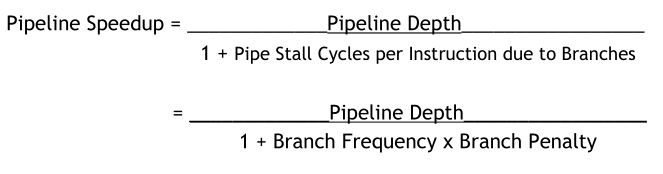
\includegraphics[scale = 0.35]{images/performace-impact-control-hazards}
    \caption{Performance impact by control hazards}
    \label{fig:performance-impact-by-control-hazards}
\end{figure}


\begin{figure}[h]
    \centering
    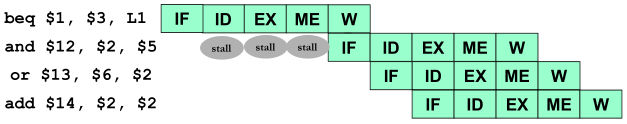
\includegraphics[scale = 0.4]{images/branch-without-forwarding}
    \caption{Branch stalls without forwarding}
    \label{fig:branch-stalls-without-forwarding}
\end{figure}

\begin{figure}[h]
    \centering
    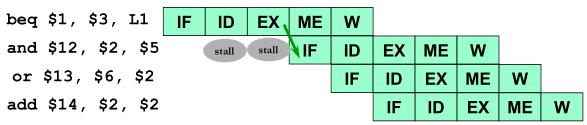
\includegraphics[scale = 0.4]{images/branch-with-forwarding}
    \caption{Branch stalls with forwarding}
    \label{fig:branch-stalls-with-forwarding}
\end{figure}

In order to reduce the speed penalty cause by the branch hazards we can use prediction techniques in order to guess
the next instruction to be executed.

\subsection{Static branch prediction}\label{subsec:static-branch-prediction}
Static branch prediction are at compile-time:
\begin{itemize}
    \item Branch always taken - No jump
    \item Branch always not taken\\ In theory always jump, but in reality we have to calculate the BTA before jumping
    and at this point there is no prediction to make (at least in the MIPS pipeline).
    \item Backward taken, forward not taken\\
    Based on the assumption that backward jumps (while and for loops) are taken and forward jumps (if statements) are
    not taken.
    \item Profile driven prediction\\
    We are going make several runs of our program and the choice is based on statistical data for each branch.
    \item Delayed Branch\\
    The compiler statically schedules and independent instruction in the branch delay slot, which is executed whether
    the branch is taken.
    %The independent instruction can belong also to the branch.
    There are three ways in which the branch delay slot can be scheduled:
        \subitem From before, the instruction in the delay slot is always executed.
        \subitem From target, this strategy is preferred when the branch is taken with high probability.
        \subitem From fall-through, this strategy is preferred when the branch is not taken with high probability. In
    this case the branch delay slot is scheduled from the not-taken fall-through path.
\end{itemize}

\begin{figure}[h]
    \centering
    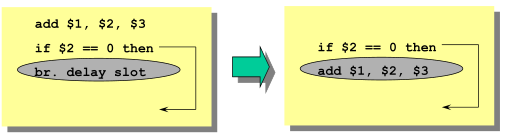
\includegraphics[scale = 0.4]{images/branch-delayed-from-before}
    \caption{Branch delayed - from before}
    \label{fig:branch-delayed-from-before}
\end{figure}

\begin{figure}[h]
    \centering
    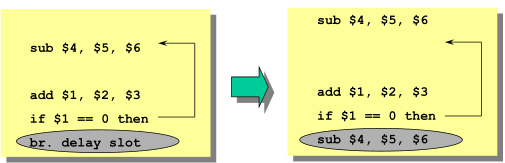
\includegraphics[scale = 0.4]{images/branch-delayed-from-target}
    \caption{Branch delayed - from target}
    \label{fig:branch-delayed-from-target}
\end{figure}

\begin{figure}[h]
    \centering
    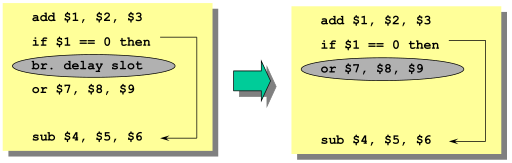
\includegraphics[scale = 0.4]{images/branch-delayed-from-fall-through}
    \caption{Branch delayed - from fall-through}
    \label{fig:branch-delayed-from-fall-through}
\end{figure}


\subsection{Dynamic branch prediction}\label{subsec:dynamic-branch-prediction}
Dynamic branch prediction happens at run-time by the hardware, and is based on two interacting mechaninsms:
\begin{itemize}
    \item Branch Outcome Predictor\\
    To predict the direction of a branch (i.e., taken or not taken).
    \subitem Branch History Table
    \item Branch Target Predictor\\
    To predict the branch target address in case of taken branch.
    \subitem Branch Target Buffer
\end{itemize}

\subsubsection{Branch Target Buffer}
The Branch Target Buffer (BTB or Branch Target Predictor) is a cache storing the predicted branch target address
for the next instruction after a branch.
We access the BTB in the IF stage using the instruction address of the fetched instruction (a possible branch) to
index the cache.

\begin{figure}[H]
    \centering
    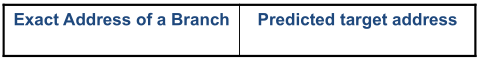
\includegraphics[scale = 0.4]{images/branch-target-buffer-entry}
    \caption{BTB entry}
    \label{fig:btb-entry}
\end{figure}

%In reality we cannot index all the possible branches since the BTB has a fixed size, the entry will not contain the
%exact address of a branch but only the last n-bits of the address, allowing the possibility for collisions.

\subsubsection{Branch History Table}
The Branch History Table (BHT or Branch Prediction Buffer) is indexed by the last k-bits of the branch address, meaning
that there are at most $2^k$ entries, with possible collisions, and each entry contains n-bits that says whether the
branch was recently taken.

\begin{figure}[H]
    \centering
    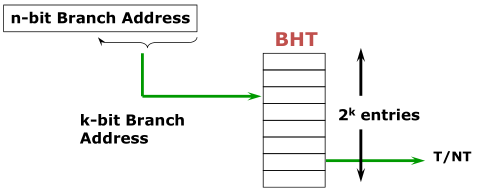
\includegraphics[scale = 0.4]{images/branch-history-table}
    \caption{Branch history table}
    \label{fig:branch-history-table}
\end{figure}

The 1-bit history table tells us if the last time the branch was taken or not taken (e.g., 0 and 1).
Differently from the profile drive prediction the BHT is updated whenever the branch is encountered.

For example:\\
0, prediction not taken, outcome not taken - no update\\
0, prediction not taken, outcome taken - update 0 to 1\\
0, prediction taken, outcome not taken - update 1 to 0\\

\begin{figure}[h]
    \centering
    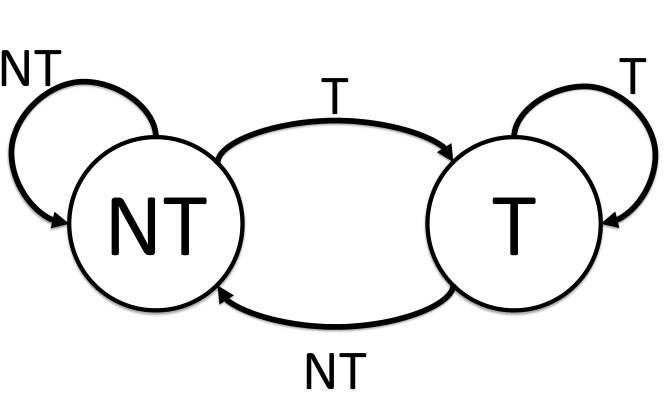
\includegraphics[scale = 0.15]{images/1-bit-BHT-automata}
    \caption{1-bit BHT automata}
    \label{fig:1-bit-BHT-automata}
\end{figure}

A misprediction occurs when:
\begin{itemize}
    \item[\textrightarrow] The prediction is incorrect for that branch
    \item[\textrightarrow] The same index has been referenced by two different branches, and the previous history
    refers to the other branch.
    To solve this problem it is enough to increase the number of rows in the BHT or to use a hashing function.
\end{itemize}

Among the n-bits BHT the 2-bit history table is the best one because it is still small in size, it allows for speedy
updates maintaining
the prediction accuracy high, but differently from the 1-bit the prediction must miss twice before it is changed.
In a loop branch we do not need to change the prediction at the last iteration, thus increasing the speed in case of
nested loop such as the ones used to inspect matrices.

\begin{figure}[h]
    \centering
    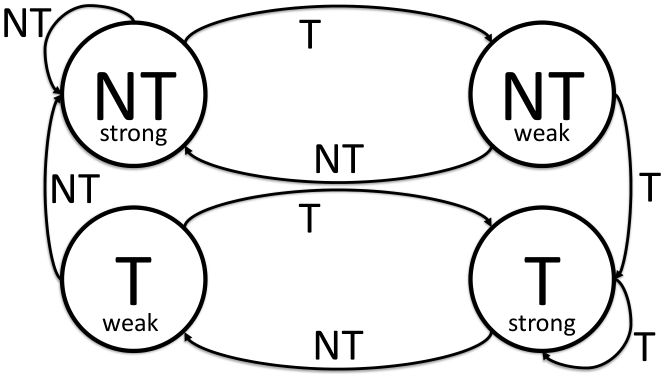
\includegraphics[scale = 0.2]{images/2-bit-BHT-automata}
    \caption{2-bit BHT automata}
    \label{fig:2-bit-BHT-automata}
\end{figure}

\begin{figure}[h]
    \centering
    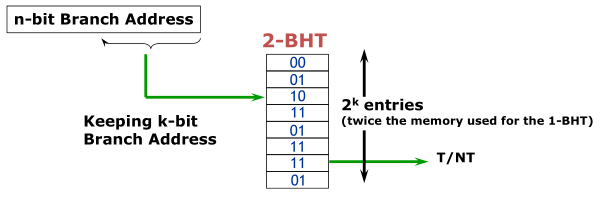
\includegraphics[scale = 0.3]{images/2-bit-BHT}
    \caption{2-bit BHT}
    \label{fig:2-bit-BHT}
\end{figure}


\subsubsection{Correlating Branch Predictor}
The idea behind is that the behaviour of recent branches are correlated, that is the recent behaviour of other
branches can influence the prediction of the current branch.
In general (m, n) correlating predictor records last m branches to choose from $2^m$ BHTs, each of which is a n-bit
predictor.
The branch prediction buffer can be indexed by
using a concatenation of low-order bits from the
branch address with m-bit global history (i.e.,
global history of the most recent m branches).

Example: a (2, 2) correlating predictor with 64 total entries;
6-bit index composed of: 2-bit global history and 4-bit low-
order branch address bits.

\begin{figure}[H]
    \centering
    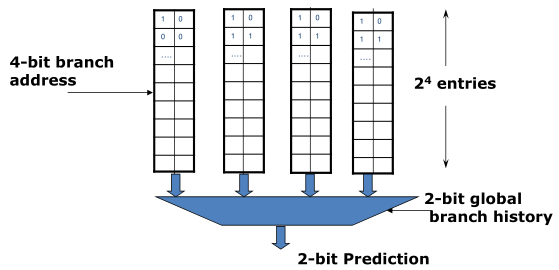
\includegraphics[scale = 0.4]{images/(2,2)-correlating-branch-predictor}
    \caption{(2,2) correlating branch predictor}
    \label{fig:(2,2)-correlating-branch-predictor}
\end{figure}

The (2,2) correlating branch predictor outperforms other predictors such as the 2-bit BHT.
    %! Author = lazza
%! Date = 03/05/2022

\section{Instruction level parallelism}\label{sec:instruction-level-parallelism}
ILP: potential overlap of execution among unrelated instructions, possible if:
\begin{itemize}
    \item no structural hazards
    \item no raw, waw, war stalls
    \item no control hazards
\end{itemize}

\begin{center}
    Pipeline CPI = Ideal pipeline CPI + Structural Stalls +\\Data Hazards Stalls + Control Stalls
\end{center}

In the MIPS architecture the only possible structural hazards, WB-ID, where a register in the RF can be both written
and read, is solved by splitting the clock cycle in rising edge (WB) and falling edge (ID).


\begin{table}[h]
    \centering
    \begin{tabular}{|p{3cm}|p{3.5cm}|}
        \toprule
        \textbf{ILP} & \textbf{PP} \\
        \midrule
        overlap individual machine operations & separate processor getting separate chuncks of the program \\
        \midrule
        transparent to the user & nontransparent to the user \\
        \midrule
        goal: speed up & goal: speed up and quality up \\
        \bottomrule
    \end{tabular}
    \caption{ILP vs Parallel Processing}
    \label{tab:ILP-vs-PP}
\end{table}


\subsection{Complex Pipeline}\label{subsec:complex-pipeline}
WAR and WAW were not possible with ADD operation with integers, but MULT and DIV operations use floating point numbers.
A new stage introduced, the ISSUE stage, that allows for high performance in presence of:
\begin{itemize}
    \item long latency or partially pipeline floating-point units
    \item multiple function and memory units
    \item memory systems with variable access time
    \item precise exception
\end{itemize}

\begin{figure}[h]
    \centering
    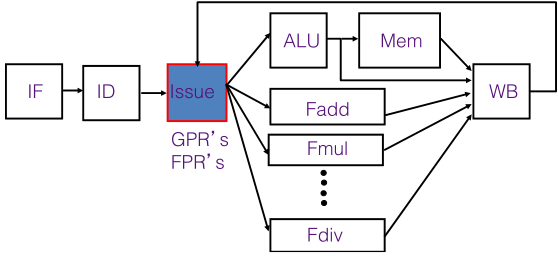
\includegraphics[scale = 0.4]{images/complex-pipeline}
    \caption{Complex pipeline}
    \label{fig:complex-pipeline}
\end{figure}

New hazards arise from variable latencies of different FUs:
\begin{itemize}
    \item Structural
    \begin{itemize}
        \item EX stage if some FPU or memory unit is not pipelined and takes more than one cycle.
        \item WB stage due to variable latencies of different functional units
    \end{itemize}
    \item Data
    \begin{itemize}
        \item WAW due to variable latencies of the FUs
    \end{itemize}
\end{itemize}

A solution would be delay the WB in order to have the same latency for all instructions but that would slow down too
much single cycle integer operations without forwarding.

\paragraph{When it is safe to issue an Instruction?} Things to consider before dispatching an instruction:
\begin{itemize}
    \item the required FU is available
    \item the input data is available
    \item it is safe to write the destination
    \item there is not a structural conflict at the WB stage
\end{itemize}

\paragraph{Assumptions} Of a general complex pipeline architecture:
\begin{itemize}
    \item all functional units are pipelined
    \item registers are read in ISSUE stage: we consider that a register is written (WB) in the first half of the clock
    cycle and read (IS) in the second half of the clock cycle
    \item no forwarding
    \item ALU operations take 1 clock cycle
    \item FP ALU operations take 2 clock cycles
    \item memory operations take 2 clock cycles
    \item write back unit has a single port
    \item instructions are fetched, decoded and issued in order
    \item an instruction will only enter the ISSUE stage if it does not cause a WAR or WAW hazard
    \item only one instruction can be issued at a time, and in the case multiple instructions are ready, the oldest
    one will go first
\end{itemize}


To reach higher performance more parallelism must be achieved, this cannot be done augmenting the CPI of the ideal
pipeline because it could create further problems with hazards.

Dependences must be detected and solved, and
instructions must be ordered (scheduled) so as to
achieve highest parallelism of execution compatible
with available resources.

Three types of dependencies:
\begin{itemize}
    \item data dependencies, RAW
    \item control dependencies
    \item name dependencies, two types:
    \begin{itemize}
        \item antidependencies, WAR
        \item output dependencies, WAW
    \end{itemize}
    Generated by the lack of registers.
\end{itemize}

Dependencies are a property of the program, while
hazards are a property of the pipeline.


The main techniques to eliminate dependencies are:
\begin{itemize}
    \item register renaming
    \item scheduling
    \begin{itemize}
        \item static, compiler
        \item dynamic, hardware
    \end{itemize}
\end{itemize}
%-> superscalar

Steps to exploit more ILP in terms of hardware optimization:
\begin{itemize}
    \item[\textrightarrow] sequential
    \begin{itemize}
        \item[$\hookrightarrow$] pipeline\\ single-issue in-order-execution
        \begin{itemize}
            \item[$\hookrightarrow$] dynamic scheduling\\ single-issue out-of-order execution
            \begin{itemize}
                \item[$\hookrightarrow$] superscalar\\ multiple-issue out-of-order execution
            \end{itemize}
        \end{itemize}
    \end{itemize}
\end{itemize}

\begin{figure}
    \centering
    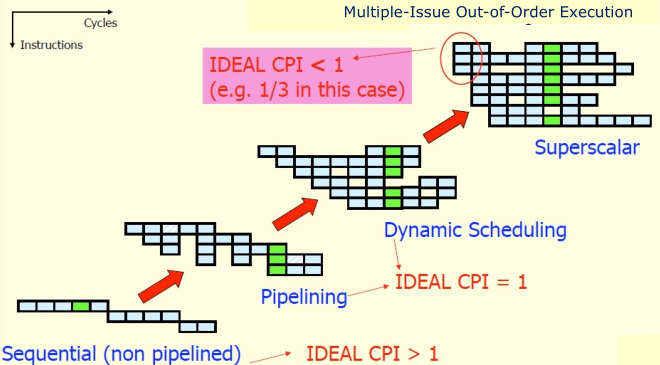
\includegraphics[scale = 0.35]{images/ILP-scheme}
    \caption{Instruction Level Parallelism}
    \label{fig:ILP-scheme}
\end{figure}

    %! Author = lazza
%! Date = 03/05/2022

\section{Static scheduling}\label{sec:static-scheduling}
Compilers can use sophisticated algorithms for code
scheduling to exploit ILP\@.
The amount of parallelism available within a \textbf{basic block}, a straight-line code sequence with no branches in
except to the entry and no branches out except at the
exit, is quite small (statistically it varies from 4 to 7 instructions).

Data dependence can further limit the amount of ILP we
can exploit within a basic block to much less than the
average basic block size.

To obtain substantial performance enhancements, we
must exploit ILP across multiple basic blocks (i.e.,
across branches).

Static detection and resolution of dependencies are accomplished by the compiler, dependencies are avoided by code
reordering.

The output of the compiler is a reordered dependency-free code, which can be processed, for example, by the VLIW (Very
Long Instruction Word) processors.

\paragraph{Limits of Static Scheduling}
\begin{itemize}
    \item unpredictable branches
    \item variable memory latency
    \item code size explosion
    \item compiler complexity
\end{itemize}

Till know we had a single-core multi-cycle parallelism, thanks to the single-issue pipelined architecture.
The single-issue architecture means we cannot aim to have an ideal CPI bigger than one.

Multi-issue architectures are the next step to improve the CPI:
\begin{itemize}
    \item Superscalar
    \item VLIW
\end{itemize}

\subsection{VLIW architectures}\label{subsec:vliw-architectures}
Each instruction word contains more than one operation, the processor can initiate multiple operations per cycle
specified completely by the compiler.
This leads to a low hardware complexity:
\begin{itemize}
    \item no scheduling
    \item reduced support of variable latency instructions
    \item single control flow (1 PC)
    \item explicit parallelism
\end{itemize}

An instruction can be a set of operations that are intended to be issued simultaneously, the VLIW has multiple
operations packed into one instruction, and each type of operation has its own slot.

\begin{figure}[h]
    \centering
    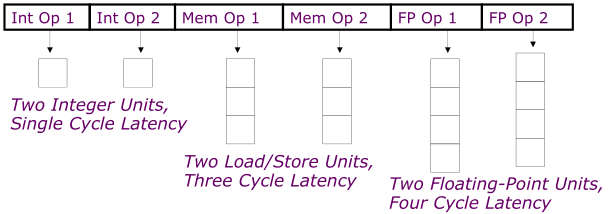
\includegraphics[scale = 0.4]{images/vliw}
    \caption{Very Long Instruction Word}
    \label{fig:vliw}
\end{figure}

This type of architecture requires guarantees of:
\begin{itemize}
    \item parallelism within an instruction does not generate RAW data hazard
    \item no data use before the data is ready, no data interlocks
\end{itemize}

Compiler responsibilities:
\begin{itemize}
    \item maximize parallel execution
    \begin{itemize}
        \item exploit ILP and LLP (Loop Level Parallelism)
        \item it is necessary to map the instructions over the machine functional units
        \item this mapping must account for time constraints and dependencies among the tasks
    \end{itemize}
    \item guarantee intra instruction parallelism
    \item avoid hazards (no interlocks), typically separates operations with explicit nops
    \item minimize the total execution time
\end{itemize}


\paragraph{Pros:}
\begin{itemize}
    \item[] simple HW
    \item[] good compilers can effectively detect parallelism
\end{itemize}
\paragraph{Cons:}
\begin{itemize}
    \item huge number of registers to keep active the FUs
    \begin{itemize}
        \item needed to store operands and results
    \end{itemize}
    \item large data transport capacity between
    \begin{itemize}
        \item FUs and register files
        \item Register files and Memory
    \end{itemize}
    \item high bandwidth between i-cache and fetch unit
    \item large code size
    \begin{itemize}
        \item use of (big) nops in the VLIW
        \item unpredictable branches have different optimal schedules that varies with branch path
    \end{itemize}
    \item knowing branch probabilities requires significant extra steps in build process due to profiling
\end{itemize}


An example of scheduling of a loop in VLIM architecture:
\begin{table}[h]
    \centering
    \begin{tabular}{c|c|c|c}
        \toprule
        operations & \textbf{ls, sd} & \textbf{add, bne} & \textbf{fadd} \\
        \midrule
        clock cycles & 3 & 1 & 4\\
        \bottomrule
    \end{tabular}
    \label{tab:}
\end{table}

\begin{figure}[h]
    \centering
    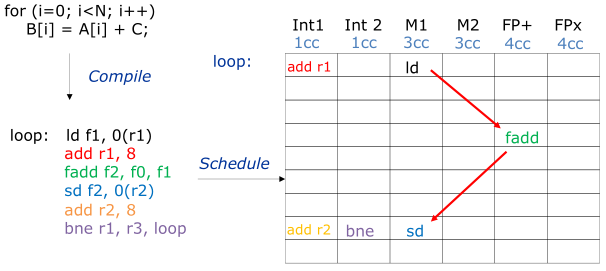
\includegraphics[scale = 0.4]{images/vliw-no-loop-unrolling}
    \caption{Loop execution on VLIM}
    \label{fig:vliw-no-loop-unrolling}
\end{figure}

Many blank lines in the scheduler corresponds to nops, leading to \(\frac{1\text{ FP ops}}{8\text{ cycles}} = 0,125\)
, which is far from our ideal CPI > 1.
To increase parallelism we use loop unrolling.

\clearpage
\subsection{Loop unrolling}
The idea is that we can extend the loop body as to include a finite number of subsequent iterations of the loop,
increasing the amount of available ILP\@.
Unrolling simply replicates the loop body multiple times, adjusting the loop termination code, by doing so the loop
\textit{overhead} decrease relatively to the loop \textit{body}.

\begin{center}
    Loop = (loop prolog + \(4\, \times\)\textit{loop body} + loop epilog) \texttimes $\, \frac{n}{4}$ iterations
\end{center}

\begin{figure}[h]
    \centering
    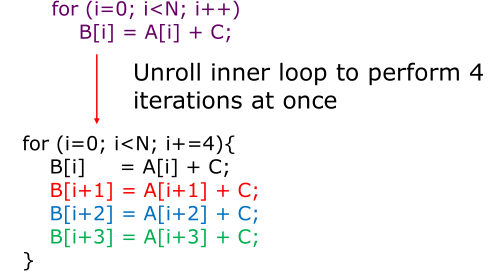
\includegraphics[scale = 0.4]{images/loop-unrolling-1}
    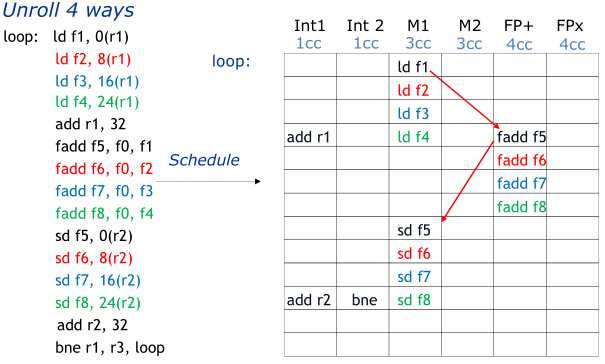
\includegraphics[scale = 0.4]{images/loop-unrolling-2}
    \caption{Loop unrolling}
    \label{fig:loop-unrolling}
\end{figure}

Note that non FP operations can have multiple schedule locations, e.g., the \verb|ld f2| could be scheduled also in
the first cycle to M2, but if does not decrease the CPI, it is recommended using a new instruction.
In this case we end up with \(\frac{4\text{ FP ops}}{11\text{ cycles}} \approx 0,36\), more than doubling the
previous result.

The \textbf{limits} of loop unrolling:
\begin{itemize}
    \item[] code size
    \item[] number of register
\end{itemize}
That is, we have an upper bound to the number of replications of the loop body, which has to be considered constant
in regard to the $\theta(n)$ loop iterations: we reduced the \textit{prolog} and \textit{epilog} of the loop by
a constant.

We can optimize the results of loop unrolling with \textbf{software pipelining}, further increasing the ILP\@.
\begin{figure}[h]
    \centering
    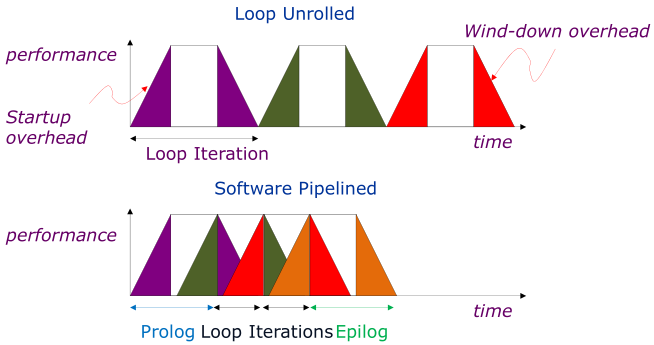
\includegraphics[scale = 0.4]{images/loop-unrolled-vs-software-pipelined-1}
    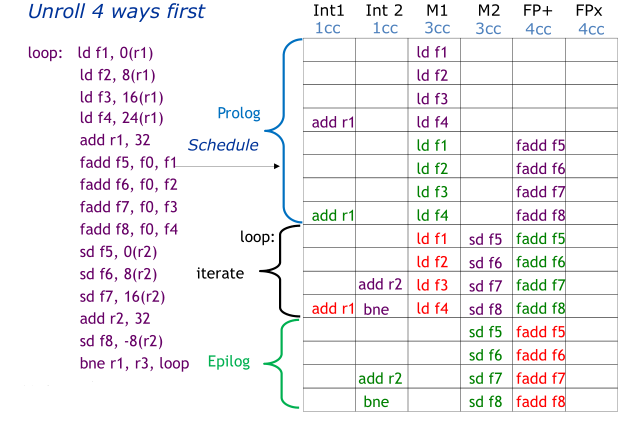
\includegraphics[scale = 0.4]{images/loop-unrolled-vs-software-pipelined-2}
    \caption{Loop unrolled vs Software pipelined}
    \label{fig:loop-unrolled-vs-sw-pipelined}
\end{figure}

\begin{center}
    Software Pipelined Loop = prolog + \textit{iterations} + epilog
\end{center}

In this case we have just one prolog and one epilog for all the loop iterations and can be considered $O(1)$ with
respect to the $n$ iterations.
For this reason we consider only the \textit{iterate} part for our performance evaluation which is \(\frac{4\text{ FP
ops}}{4\text{ cycles}} = 1\).

\textbf{Note:} in case of short loops, loop unrolling looses performance due to the costs of starting and closing the
iterations.

\clearpage
\subsection{Trace Scheduler}\label{subsec:trace-scheduler}
Loop unrolling is useful but does not cover other type of branches that limit the basic \textbf{block size} in
control-flow intensive irregular code.
In these cases is difficult to find ILP in individual basic blocks.

Trace scheduling focus on traces:
\begin{itemize}
    \item a loop-free sequence of basic blocks embedded in the control flow graph
    \item it is an execution path which can be taken for some set of inputs
    \item the chances that a trace is actually executed depends on the input set that allows its execution
\end{itemize}

\textbf{Note:} a trace may include branches but not loops.

\paragraph{Algorithm} Idea, some traces are executed much more frequently than others:
\begin{itemize}
    \item pick string of basic blocks, a trace, that represents most frequent branch path
    \item use profiling feedback or compiler heuristics to find common branch paths
    \item schedule whole "trace" at one
    \item add fixup code to cope with branches jumping out of trace
\end{itemize}
\begin{figure}[h]
    \centering
    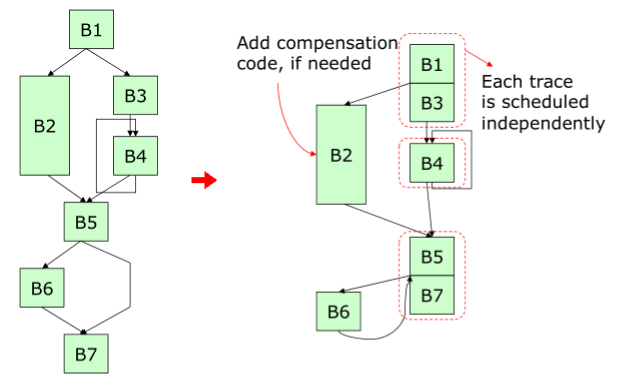
\includegraphics[scale = 0.45]{images/trace-scheduling}
    \caption{Trace scheduling}
    \label{fig:trace-scheduling}
\end{figure}

For example we suppose that \{B1, B3, B4, B5, B7\} is the most frequently executed path, therefore the traces are
\{B1, B3\}, \{B4\} and \{B5, B7\}.\\
\textbf{Note:} Traces are scheduled as if they were basic blocks, by removing control hazards we increase ILP\@.

\paragraph{Problems} Compensation codes are difficult to generate, especially entry points (of a different path).
In addition to need of compensation codes there are
restrictions on movement of a code in a trace:
\begin{itemize}
    \item \textbf{dataflow} of the program must not change, it is guaranteed to be correct by maintaining:
    \begin{itemize}
        \item data dependencies
        \item control dependencies
    \end{itemize}
    \item the exception behaviour must be preserved
\end{itemize}


\paragraph{Solutions}There are two approaches to eliminate control dependency:
\begin{itemize}
    \item use of \textbf{predicate} instructions (Hyperblock scheduling)
    \item use of \textbf{speculative} instructions (Speculative Scheduling), and speculatively move an instruction
    before the branch.
\end{itemize}

\begin{figure}[h]
    \centering
    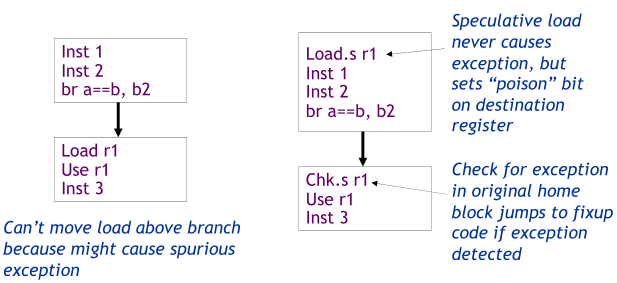
\includegraphics[scale = 0.4]{images/speculative-instruction}
    \caption{Speculative instruction}
    \label{fig:speculative-instruction}
\end{figure}

\begin{figure}[h]
    \centering
    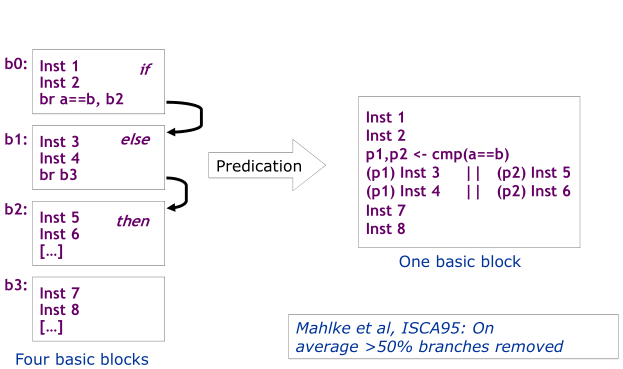
\includegraphics[scale = 0.4]{images/predicated-execution}
    \caption{Predicated execution}
    \label{fig:predicated-execution}
\end{figure}

Rotating Register Files


\clearpage
\subsection{Dynamic scheduling}\label{subsec:dynamic-scheduling}

The hardware reorders the instruction execution to reduce pipeline
stalls while maintaining data flow and exception behavior.
•
Main advantages:
– It enables handling some cases where dependences are
unknown at compile time
– It simplifies the compiler complexity
– It allows compiled code to run efficiently on a different pipeline.
•
Those advantages are gained at a cost:
– A significant increase in hardware complexity,
– Increased power consumption
– Could generate imprecise exception

Basically: Instructions are fetched and issued in program order (in-
order-issue)
•
Execution begins as soon as operands are available
– possibly, out of order execution – note: possible even with
pipelined scalar architectures.
•
Out-of order execution introduces possibility of WAR, WAW data
hazards.
•
Out-of order execution implies out of order completion unless there
is a re-order buffer to get in-order completion


    %! Author = lazza
%! Date = 03/05/2022

\subsection{Dynamic Scheduling}\label{subsec:dynamic-scheduling}

Scoreboard algo for dynamic scheduling

when is it safe to Issue an instruction slide 13
-
-
-
-

scoreboard manages commits to registers

RAW detected in ID stage, ID stage divided in two:
- instruction decode
- read registers

Scoreboard:
RAW ID stalls
WAR WB stalls
WAW not issued (stall the issue) - register renaming not used

techniques:
- register renaming

Scoreboard control structure:
1. instruction status, tells witch istr is being executed
2. functinal status, state of the functional unit
3. register result status, indicated which functional unit will write each register.

Qj and Qk tells who is going to provide the data in terms of functional unit (if not available yet)
Rj and Rk tells if the data is ready or not, prevents WAR

ADDD, DIVD, MULTD what D stands for?

in-order issue
out-of-order read
out-of-order write

-----

Tomasulo algo

load and store treated as integer FU

Common Data Bus - serialized access to write back
CDB provides values before they are saved into registers (somewhat similar to path forwarding)

FP floating point?

Reservation Station RS components
-
-
-
\ldots

STAGES
- issue
-
-

V value
Q pointer

LD: 1 cc to integer operation (offset + base address) and 1 cc to access the memory = 2 cc for Execution Completion + 1 cc to commit in the CDB

R(F4) = F4 value, register f4 Renamed

in-order issue
out-of-order execution
out-of-order write

try to do exercise on the slides

in case of concurrent writes choose the one that belongs to the critical path.

Scoreboard vs Tomasulo:
- structural hazards in scoreboard
- lack of forwarding in scoreboard


    %! Author = lazza
%! Date = 03/05/2022


Exception handling

definitions
exception :
interrupt : external of internal event that needs to be processed by another program (the interrupt handler), at the end resume normal execution

External async events:
- input output device-request
- timer expiration
- power disruptions, hardware failure

Internal sync event:
- undefined opcode, privileged instruction
- arithmetic overflow, FPU exeception
- misaligned memory access
- virtual memory exceptions: page faults, TLB misse, protection violations
- traps: system calls, e.g., jumps into kernel

Exception classes:
- synchronous vs asynchronous, asynch caused by devices external to the CPU and memory and can be handled easily
- user requested vs coerced, user requested are predictable: treated as exceptions because they use the same mechanism that are used
to save and restore the state;
handled after the instruction has completed.
Coerced are caused by some HW event not under control of the program.
- user maskable vs user nonmaskable
- within vs between instructions
- resume vs terminate

For the exam study difference between pairs.

Invoking the interrupt handler:
- terminate exec of instr till PC-4
- store the PC in EPC register, exception program counter
- disable other interrupts and transfers control to a designated interrupt running in the kernel mode

In the cpu we have two modes: user-mode and kernel-mode (unstoppable).

precise interrupts
- easy handled

Exception handling in the 5-stage pipeline

    %! Author = lazza
%! Date = 06/05/2022

\section{HW speculation}\label{sec:hw-speculation}
HW-based speculation combines three ideas:
\begin{description}[noitemsep]
    \item[Dynamic Branch Prediction] to choose which instruction to execute
    \item[Dynamic Scheduling] supporting out-of-order execution but in-order commit to prevent any irrevocable
    actions (such as register update or taking exception) until an instruction commits
    \item[Speculation] To execute instructions before control dependencies are solved
\end{description}
The idea is allowing instruction to execute freely and out-of-order, based on speculation, but allow to update the RF
or the memory only when an instruction is no longer speculative.

Mechanisms are necessary to handle incorrect speculation, hardware speculation extends dynamic scheduling beyond a
branch, i.e., behind the basic blocks.

\subsection{Reorder buffer}\label{subsec:reorder-buffer}
A buffer that holds instruction results before they are committed.
When an instruction complete execution, the results are placed into ROB, which holds the instructions in FIFO order,
exactly as issued.
The result in the ROB buffer are tagged, they are used instead of the reservation stations, supplying operands to
other instruction between execution and commit.
The instruction at the \textbf{head} of ROB can safely commit, all its predecessor have already committed.

\begin{figure}[h]
    \centering
    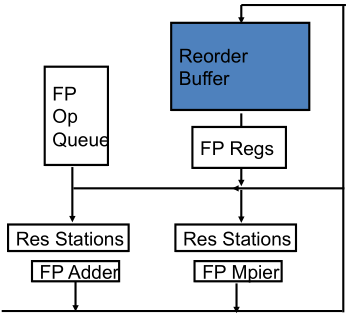
\includegraphics[scale = 0.4]{images/reorder-buffer}
    \caption{ROB}
    \label{fig:rob}
\end{figure}

\paragraph{Separating Completion from Commit} Re-order buffer holds the register result from completion until commit:
\begin{itemize}[noitemsep]
    \item[-] entries are allocated in program order during decode
    \item[-] it buffers completed values and exception state until commit point
    \item[-] completed values can be used by dependents before committed (bypassing)
    \item[-] each entry holds a program counter, instruction type, destination register specifier and value if any,
    and exception status
\end{itemize}

\paragraph{Memory reordering} It needs special data structures:
speculative store address and data buffers, speculative load address and data buffers.

\paragraph{Precise interrupts and Speculation} If a speculation is wrong, we need to be able to back and restart
execution to a point before out incorrect prediction (e.g., branch prediction), it happens the same as precise
exceptions.
The recovery technique for both is \textbf{in-order commit}.


\subsection{Speculative Tomasulo}\label{subsec:speculative-tomasulo}
\subsubsection{Stages}
\begin{description}
    \item[Issue] get instruction from FP Op Queue.\\
    If the reservation station \textcolor{red}{and reorder buffer slot} are free: issue instruction, send
    operands, \textcolor{red}{reorder buffer number for destination.}
    \item[Execution] operate on operands when ready.\\
    If not ready, watch CDB for result: when both are in the reservation station, execute then check for RAW.
    \item[Write result] finish execution.\\
    Write on Common Data Bus to all awaiting FUs \textcolor{red}{and reorder buffer}.
    Mark the reservation station available.
    \item[Commit] \textcolor{red}{update register with reorder result}.\\
    \textcolor{red}{When and instruction at the head of ROB and the result is present, update the register or memory,
        and remove instruction from ROB. In case of mispredicted branch flush the reorder buffer.}\\
    Three types of commit:
    \begin{itemize}[noitemsep]
        \item normal commit
        \item store commit
        \item flush results if incorrect branch prediction
    \end{itemize}
\end{description}

\begin{figure}
    \centering
    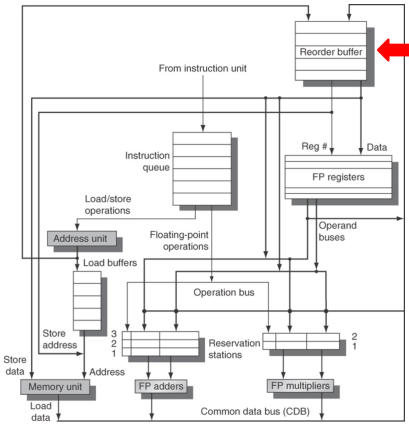
\includegraphics[scale = 0.5]{images/speculative-tomasulo}
    \caption{Speculative tomasulo}
    \label{fig:speculative-tomasulo}
\end{figure}

\subsubsection{ROB entries}
Each ROB entries contains four fields:
\begin{description}
    \item[Instruction type field] indicates whether instruction
    is a branch (no destination result), a store (has
    memory address destination), or a load/ALU
    (register destination)
    \item[Destination field] supplies register number (for
    loads and ALU instructions) or memory address (for
    stores) where results should be written
    \item[Value field] holds value of result until
    instruction commits
    \item[Ready filed] indicates that instruction has
    completed execution, ready to commit
\end{description}

\subsubsection{ROB extension}
The addition of the reorder buffer introduces changes in tomasulo:
\begin{itemize}[noitemsep]
    \item ROB completely replaces store buffers
    \item renaming function of reservation stations completely replaced
    \item reservation stations now only queue operations (and operands) to FUs between issue and execution.
    \item results are tagged with ROB entry number rather than with RS number, ROB entry must be tracked in the
    reservation stations
    \item all instructions excluding incorrectly predicted branches (or incorrectly speculated loads) commit when
    reaching head of ROB
    \item when a incorrectly predicted branch reaches the head, ROB is flushed, execution restarts at correct
    successor of branch \textrightarrow speculative active are easily undone
    \item processor with ROB can dynamically speculate while maintaining a precise interrupt model
\end{itemize}


    %! Author = lazza
%! Date = 07/05/2022

\section{Explicit register renaming}\label{sec:register-renaming}
Tomasulo provides \textit{implicit} register renaming by the means of reservation stations or ROB\@.
Now we introduce \textit{explicit} register renaming: use a physical register file that is larger than the number of
registers specified by the ISA\@.

Idea: allocate a new physical destination register for every instruction that writes:
\begin{itemize}[noitemsep]
    \item removes WAW, WAR hazards
    \item allows out-of-order completion (like tomasulo)
    \item similar to SSA, Static Single Assignment transformation done the compiler
\end{itemize}

\paragraph{Mechanism} Keep a translation table:
\begin{itemize}[noitemsep]
    \item map ISA \textit{logical} register to physical register
    \item when a register is written, replace the map entry with new register from freelist
    \item physical register becomes free when not used by any active instructions
\end{itemize}

\paragraph{Unified physical register file}
\begin{itemize}
    \item rename all architectural (logical) registers into a single physical register file during decode, no register
    values read
    \item FUs read and write from single unified register file holding committed and temporary registers in execution
    \item commit only updates mapping of architectural register to physical register, no data movement
\end{itemize}

\paragraph{HW register renaming}
\begin{description}
    \item[Renaming map] simple data structure that supplies the physical register number of the register that
    currently corresponds to the requested architectural register
    \item[Instruction commit] update permanently the renaming table to indicate that the physical register holding
    the destination values corresponds to the actual architectural register
    \item[ROB] Use reorder buffer to enforce in-order commit
\end{description}

\subsection{Explicit renaming - Scoreboard}\label{subsec:explicit-renaming---scoreboard}
\subsubsection{Stages}
\begin{description}
    \item[Issue] decode instructions and check for structural hazards \textcolor{red}{and allocate new physical
    register for result}:
    \begin{itemize}[noitemsep]
        \item[-] instructions issued in program order (for hazard checking)
        \item[-] \textcolor{red}{don't issue if there are no free physical registers}
        \item[-] don't issue if there's a structural hazard
    \end{itemize}
    \item[Read operands] wait until there are no more hazards, then read operands.
    All real dependencies solved in this stage, since we wait for instructions to write data back.
    \item[Execution] operate on operands.
    The functional unit begins execution upon receiving operands.
    When the result is ready, it notifies the scoreboard.
    \item[Write result] finish execution
\end{description}
\textbf{Note:} \textcolor{red}{no check for WAR and WAW hazards.}

\subsection{Register renaming vs ROB}\label{subsec:register-renaming-vs-rob}
\begin{itemize}[noitemsep]
    \item[-] instruction commit simpler than with ROB
    \item[-] deallocating register more complex
    \item[-] dynamic mapping or architectural to physical registers complicates design and debugging.
\end{itemize}



    %! Author = lazza
%! Date = 07/05/2022
\section{ILP limits}\label{sec:ilp-limits}
\subsection{Superscalar}\label{subsec:superscalar}
Superscalar execution allows multiples-issue and out-of-order execution.
A superscalar processor can execute more than one instruction during a clock cycle by simultaneously
dispatching multiple instructions to different execution units on the processor.
It therefore allows more throughput than would otherwise be possible at a given clock rate.
Each execution unit is not a separate processor (or a core if the processor is a multicore processor), but an
execution resource within a single CPU such as an arithmetic logic unit.
In Flynn's taxonomy, a single-core superscalar processor is classified as an SISD processor, though a single-core
superscalar processor that supports short vector operations could be classified as SIMD (single instruction stream,
multiple data streams).
A multicore superscalar processor is classified as an MIMD processor (multiple instruction streams, multiple data streams).
While a superscalar CPU is typically also pipelined, superscalar and pipelining execution are considered different
performance enhancement techniques.
The former executes multiple instructions in parallel by using multiple execution units, whereas the latter executes
multiple instructions in the same execution unit in parallel by dividing the execution (instruction) unit into
different phases.

\paragraph{Key requirements}
\begin{description}
    \item[-] Fetching more instructions per clock cycle: no major problem provided the instruction cache can sustain
    the bandwidth and can manage more requests at the same time.
    \item[-] Decide on data and control dependencies: dynamic scheduling and dynamic branch prediction
\end{description}

\paragraph{Beyond CPI = 1} 
\begin{itemize}[noitemsep]
    \item issue multiple instruction per clock-cycle
    \item varying number of instruction per cycle (1 to 8)
    \item scheduled by the compiler or HW
\end{itemize}
\[CPI_{ideal} =\frac{1}{issue-width}\]


With single-issue ILP we can be reach an ideal CPI =~1.
With superscalar execution our \textit{ideal} CPI can decrease furthermore.

\subsection{Assumptions}\label{subsec:assumptions}
The ideal machine must have:
\begin{description}
    \item[Register renaming] infinite virtual registers and all WAW and WAR hazards are avoided
    \item[Branch prediction] perfect, no mispredictions
    \item[Jump prediction] all jumps perfectly predicted, machine with perfect speculation and an unbounded buffer of
    instructions available
    \item[Memory address alias analysis]\footnote{Alias analysis is a technique used to determine if a storage location may be accessed in more than one way} addresses are know and a store can be moved before a load provided the 
    addresses not equal 
    \item[One cycle latency for all instructions] unlimited number of instructions issued per clock cycle
\end{description}

\subsection{Limits on window size}\label{subsec:limits-on-window-size}
Dynamic analysis is necessary to approach
perfect branch prediction (impossible at compile
time!).
A perfect dynamic-scheduled CPU should:
\begin{itemize}[noitemsep]
    \item[-] Look arbitrarily far ahead to find set of instructions to
    issue, predict all branches perfectly
    \item[-] Rename all registers uses (no WAW, WAR hazards);
    \item[-] Determine whether there are data dependencies
    among instructions in the issue packet, rename if
    necessary
    \item[-] Determine if memory dependencies exist among
    issuing instructions, handle them
    \item[-] Provide enough replicated functional units to allow all
    ready instructions to issue.
\end{itemize}
Size affects the number of comparisons necessary to determine
RAW dependencies.
The number of comparisons to evaluate for data dependencies among n register-to-register
instructions in the issue phase is \(n^2 - n\).


\end{document}
